
	El filtro de Kalman obtiene la mejor estimación en el sentido del error cuadrático medio. Esto quiere decir que cuanto mayor sea la varianza de el ruido de proceso, mas importancia le dará a las mediciones. De la misma manera, cuanto mayor sea la varianza del ruido de medición, mayor importancia le dará al modelo en el espacio de estados para poder realizar la estimación. El objetivo de este punto es ver como se modifica la estimación modificando la magnitud de la matriz de covarianza del ruido de proceso.
	
	En las figuras \ref{fig:ej5r1} y \ref{fig:ej5r2} se observan las estimaciones de las trayectoras para una matriz de covarianza del ruido de proceso $100$ veces mayor y $100$ veces menor a la original, respectivamente. Puede observarse que en el caso de la matriz mayor, el algoritmo le da menos importancia al modelo, y mas a las mediciones. De esta manera, se deja llevar mas por las mediciones y la variabilidad de la trayectoria respecto de la real es mayor que en el caso en que se usa una matriz menor.
	
	\begin{figure}[H]
		\centering
		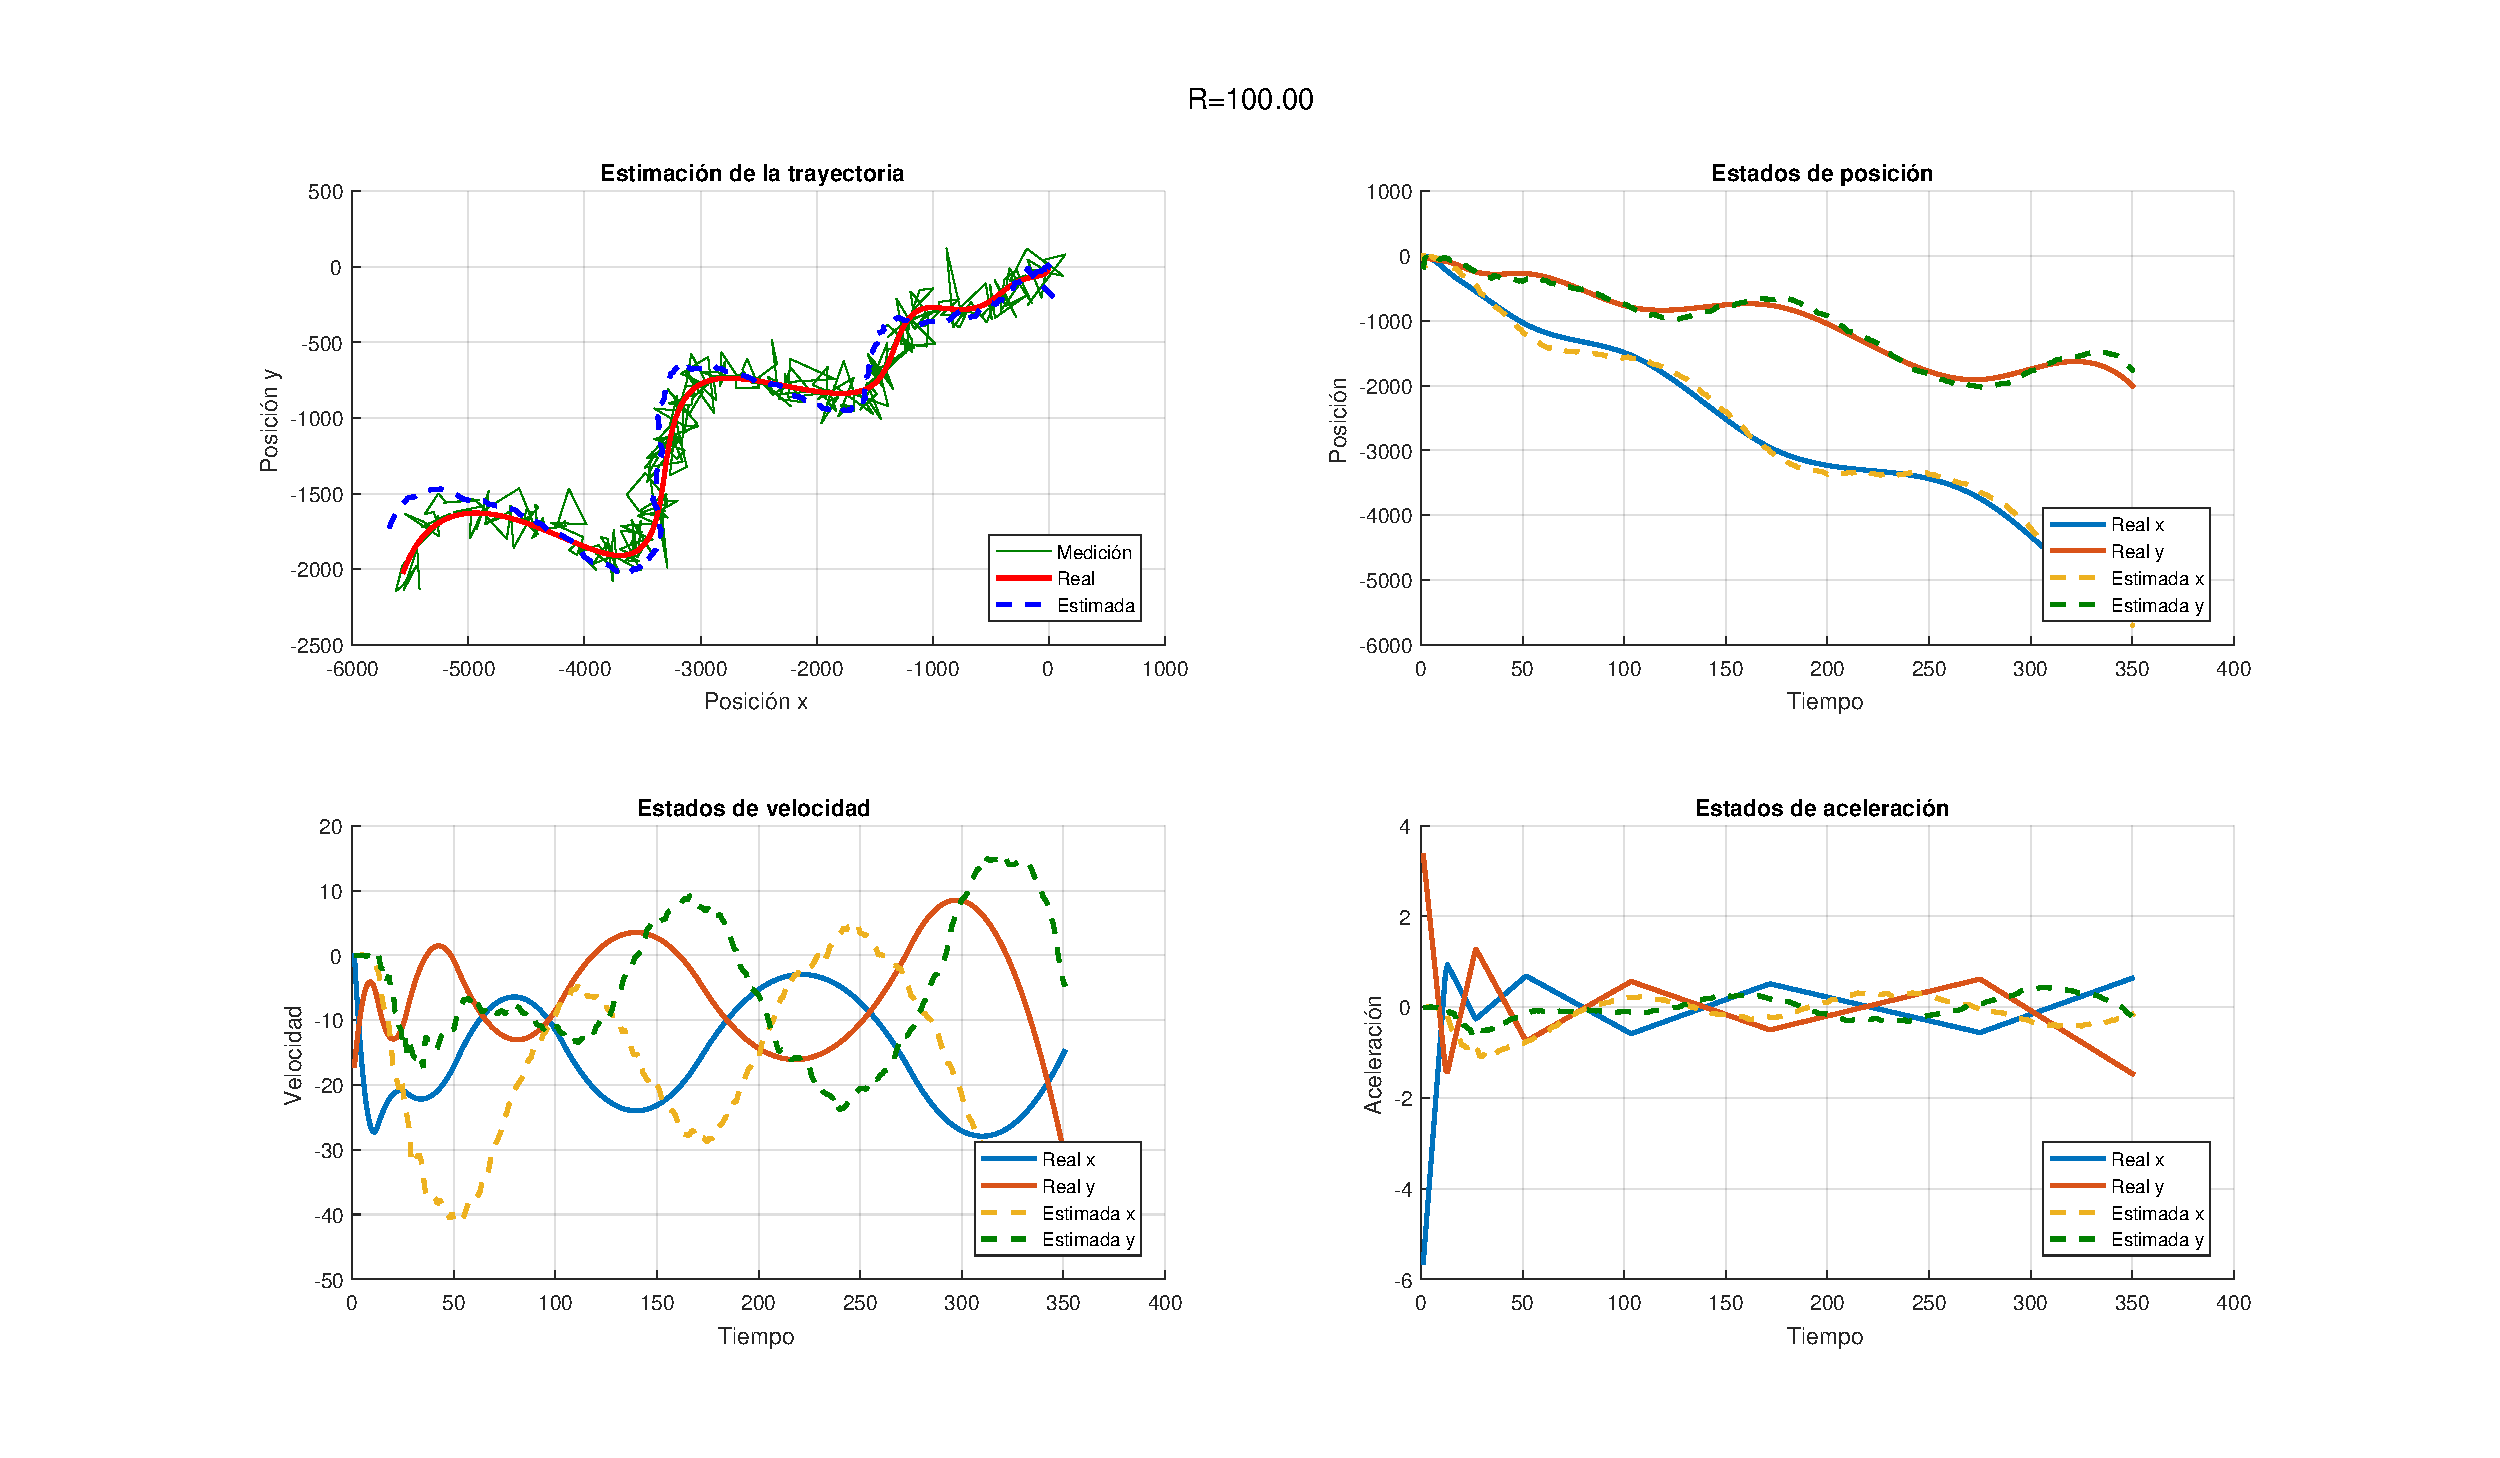
\includegraphics[width=1.0\textwidth,keepaspectratio]{Figuras/graf_ej6_R1.pdf}
		\caption{Estimación de Trayectoria - Matriz de Covarianza Mayor}
		\label{fig:ej5r1}
	\end{figure}
	
	\begin{figure}[H]
		\centering
		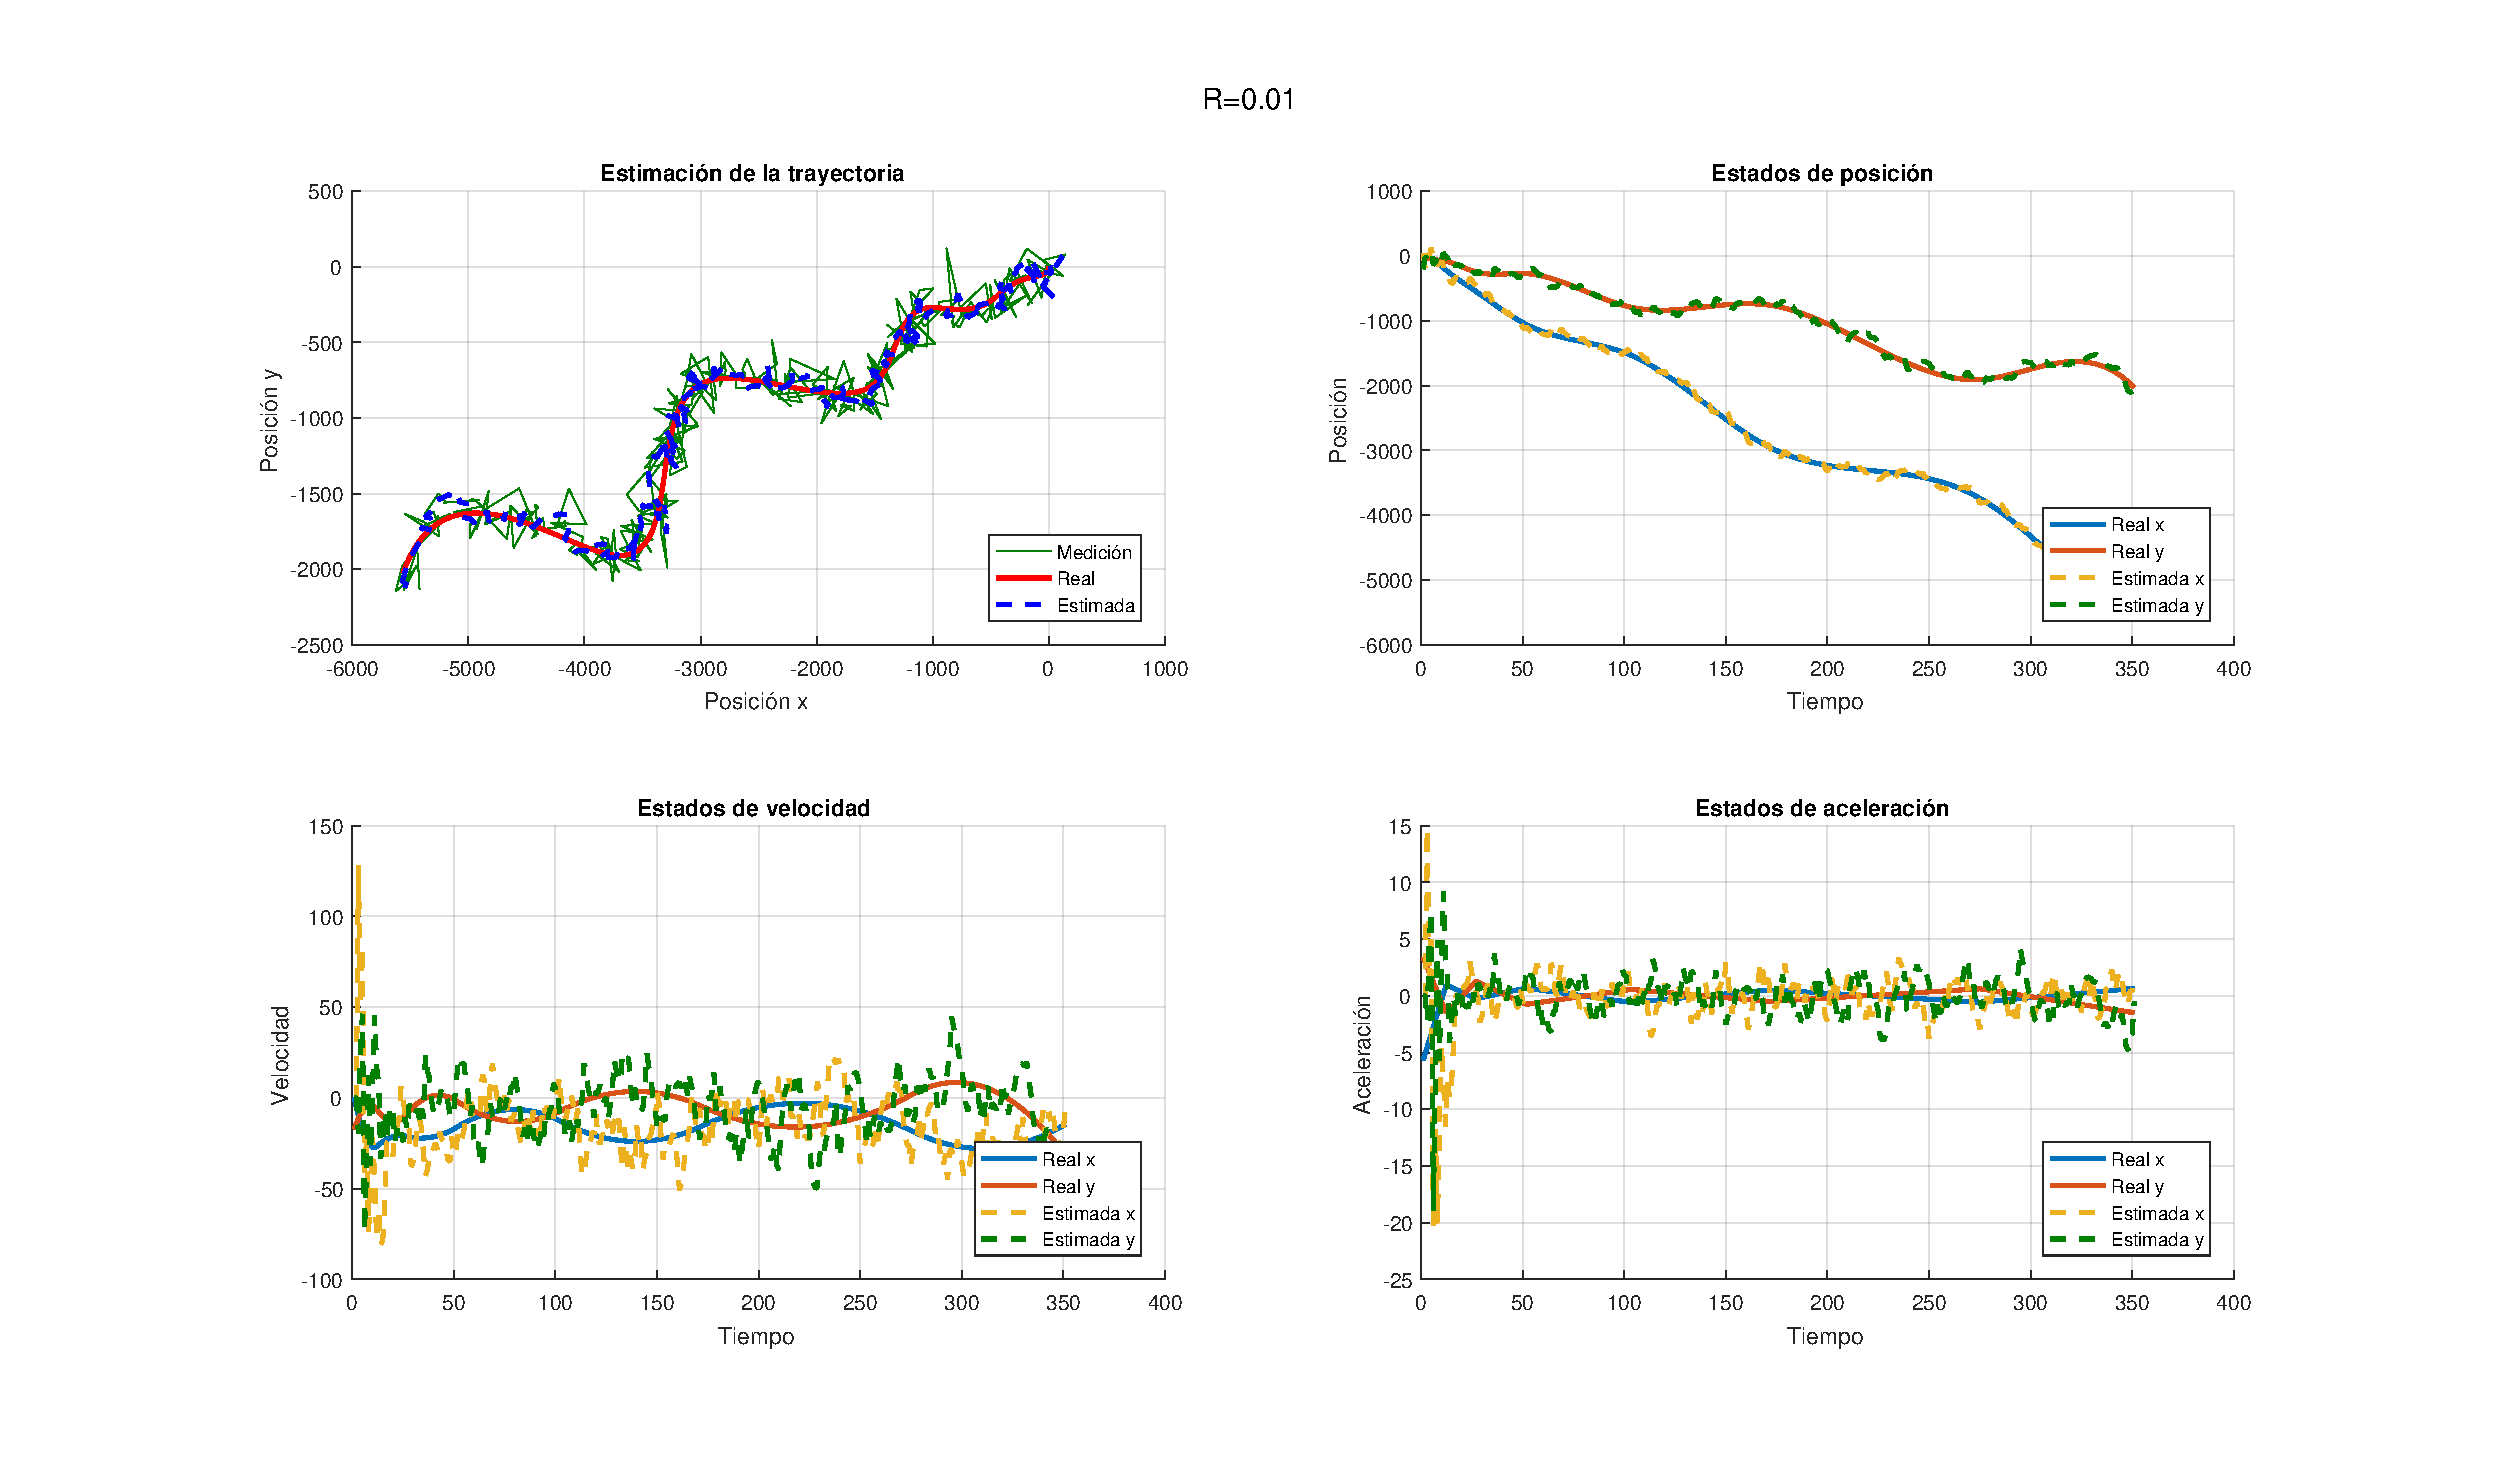
\includegraphics[width=1.0\textwidth,keepaspectratio]{Figuras/graf_ej6_R2.pdf}
		\caption{Estimación de Trayectoria - Matriz de Covarianza Menor}
		\label{fig:ej5r2}
	\end{figure}
	
	En las figuras \ref{fig:ej5r1_innov} y \ref{fig:ej5r2_innov} se observan las autocorrelaciones de las innovaciones. Puede observarse que cuanto mayor sea la matriz de ruido de proceso, el proceso es menos blanco, y por consiguente, se concluye que la estimación es peor.
	
	\begin{figure}[H]
		\centering
		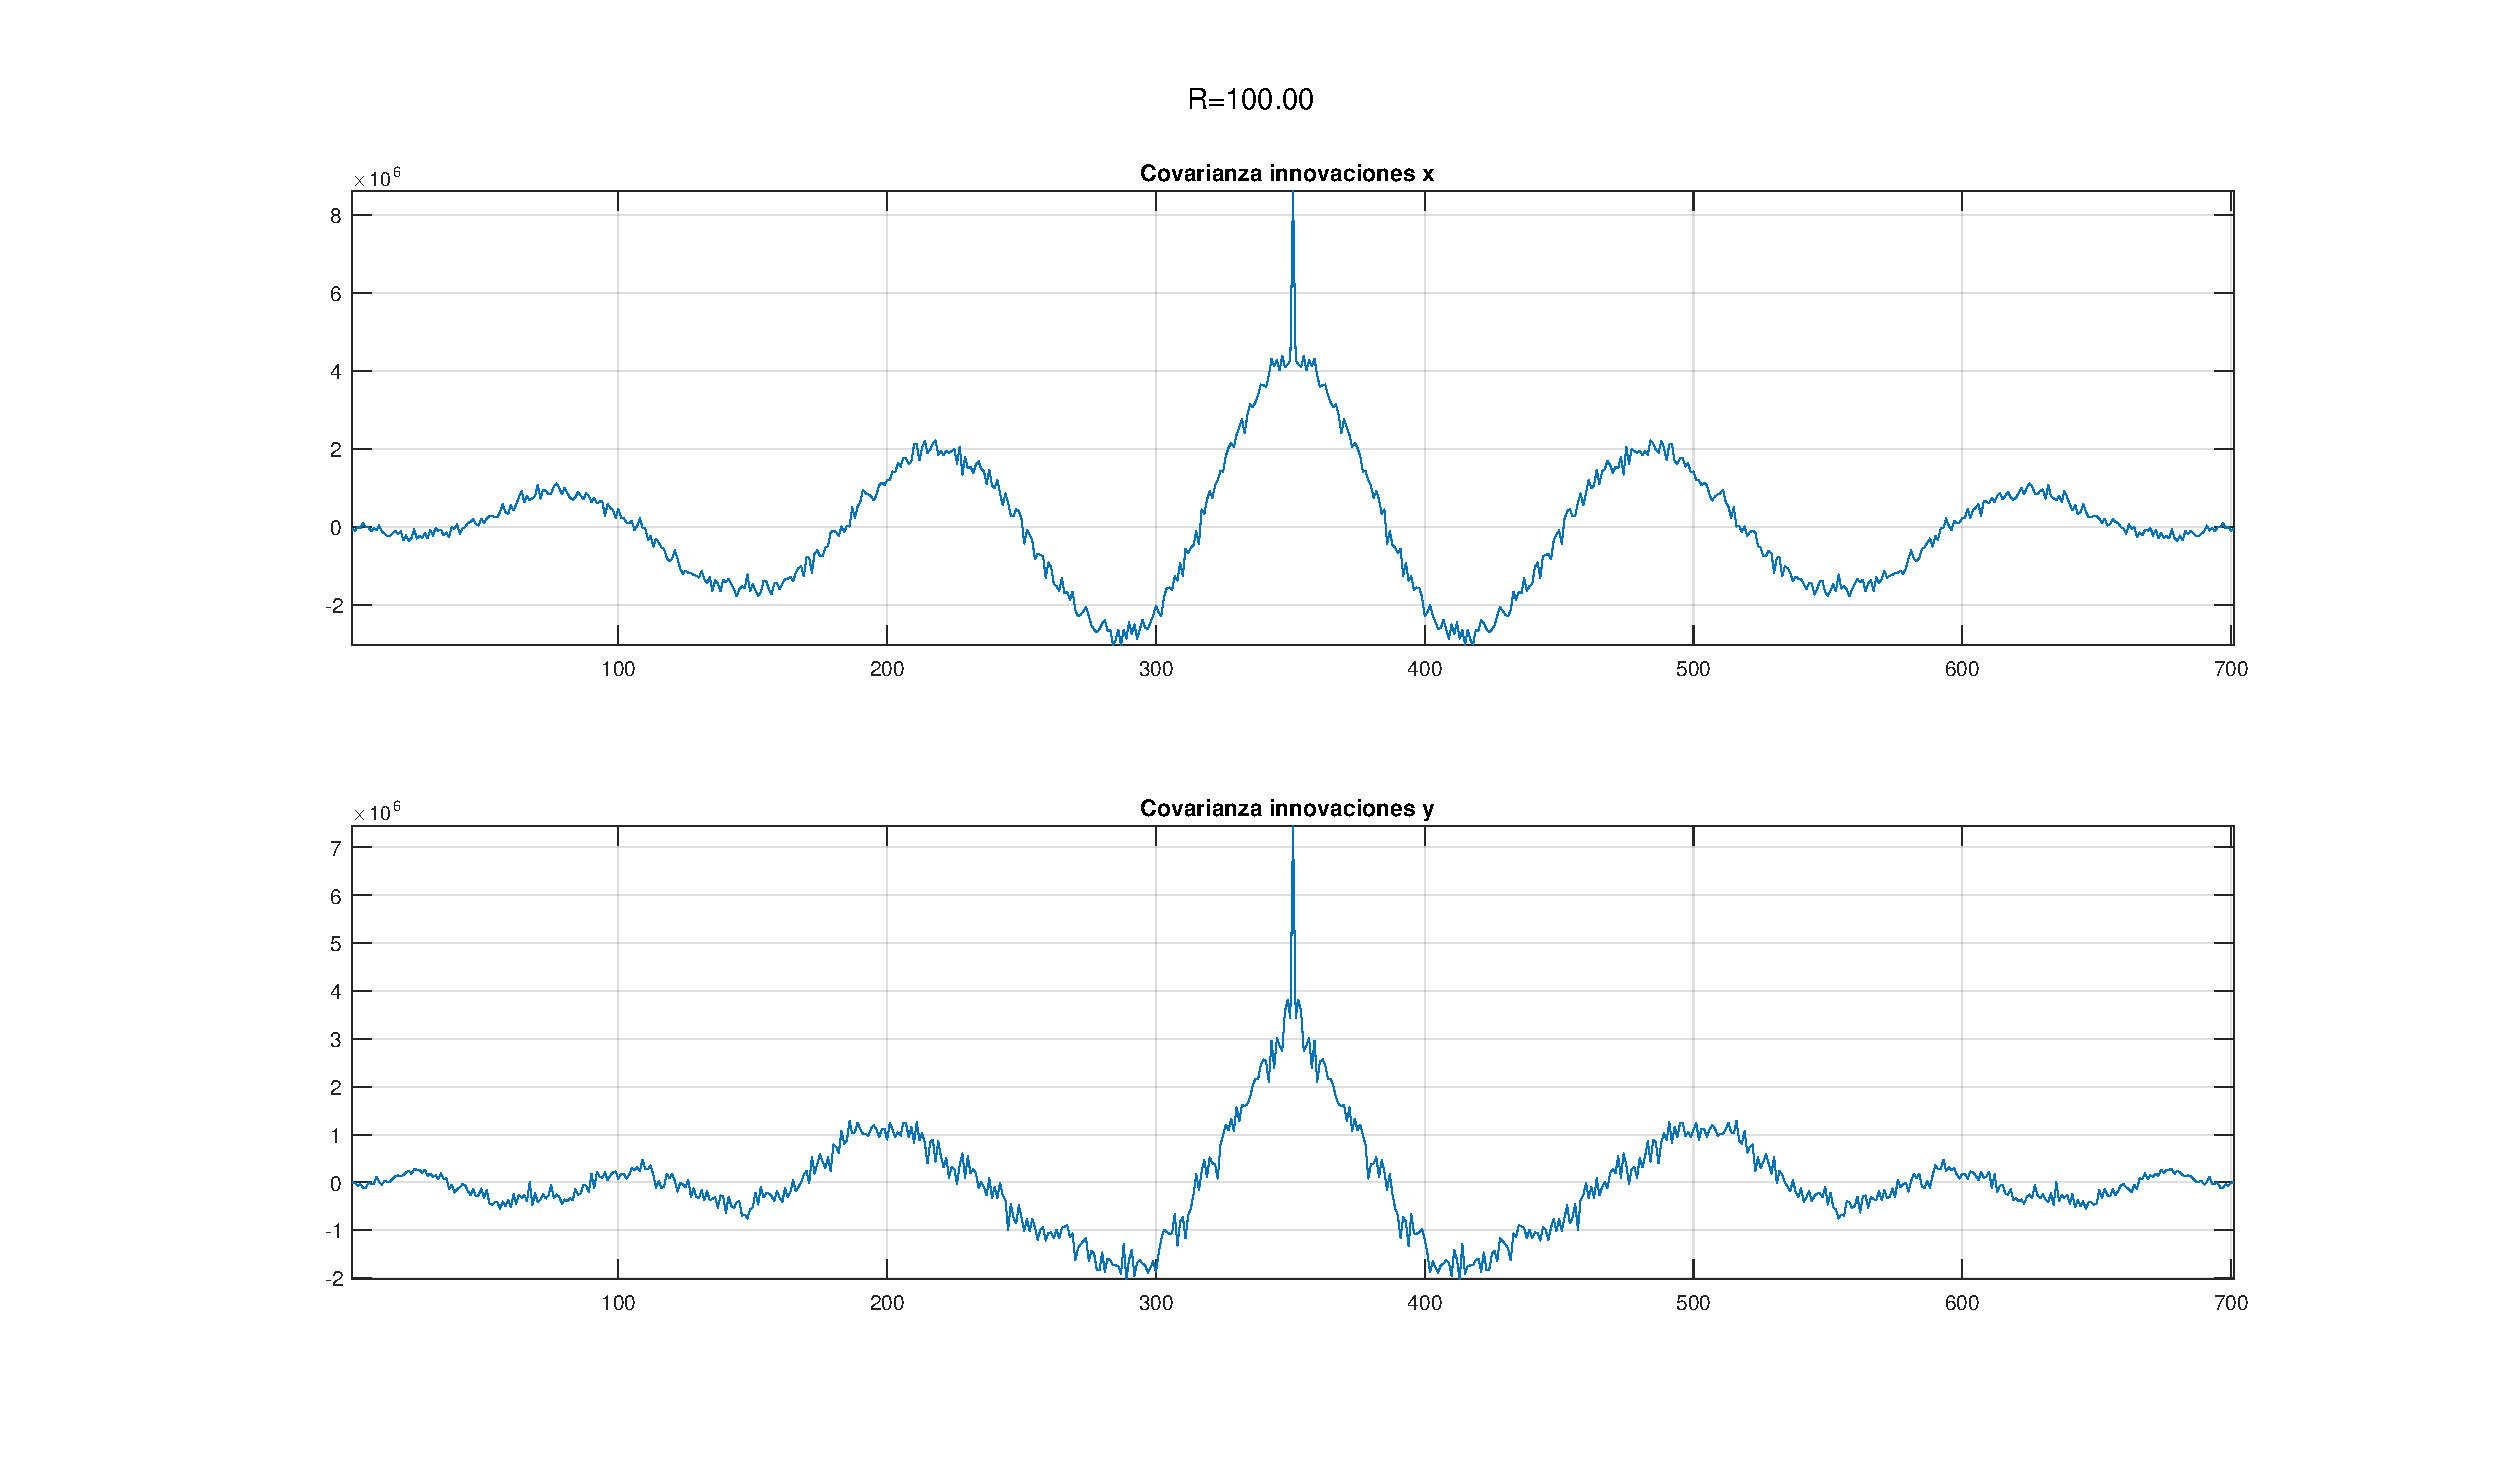
\includegraphics[width=1.0\textwidth,keepaspectratio]{Figuras/covinn_ej6_R1.pdf}
		\caption{Autocorrelación de Innovaciones - Matriz de Covarianza Mayor}
		\label{fig:ej5r1_innov}
	\end{figure}
	
	\begin{figure}[H]
		\centering
		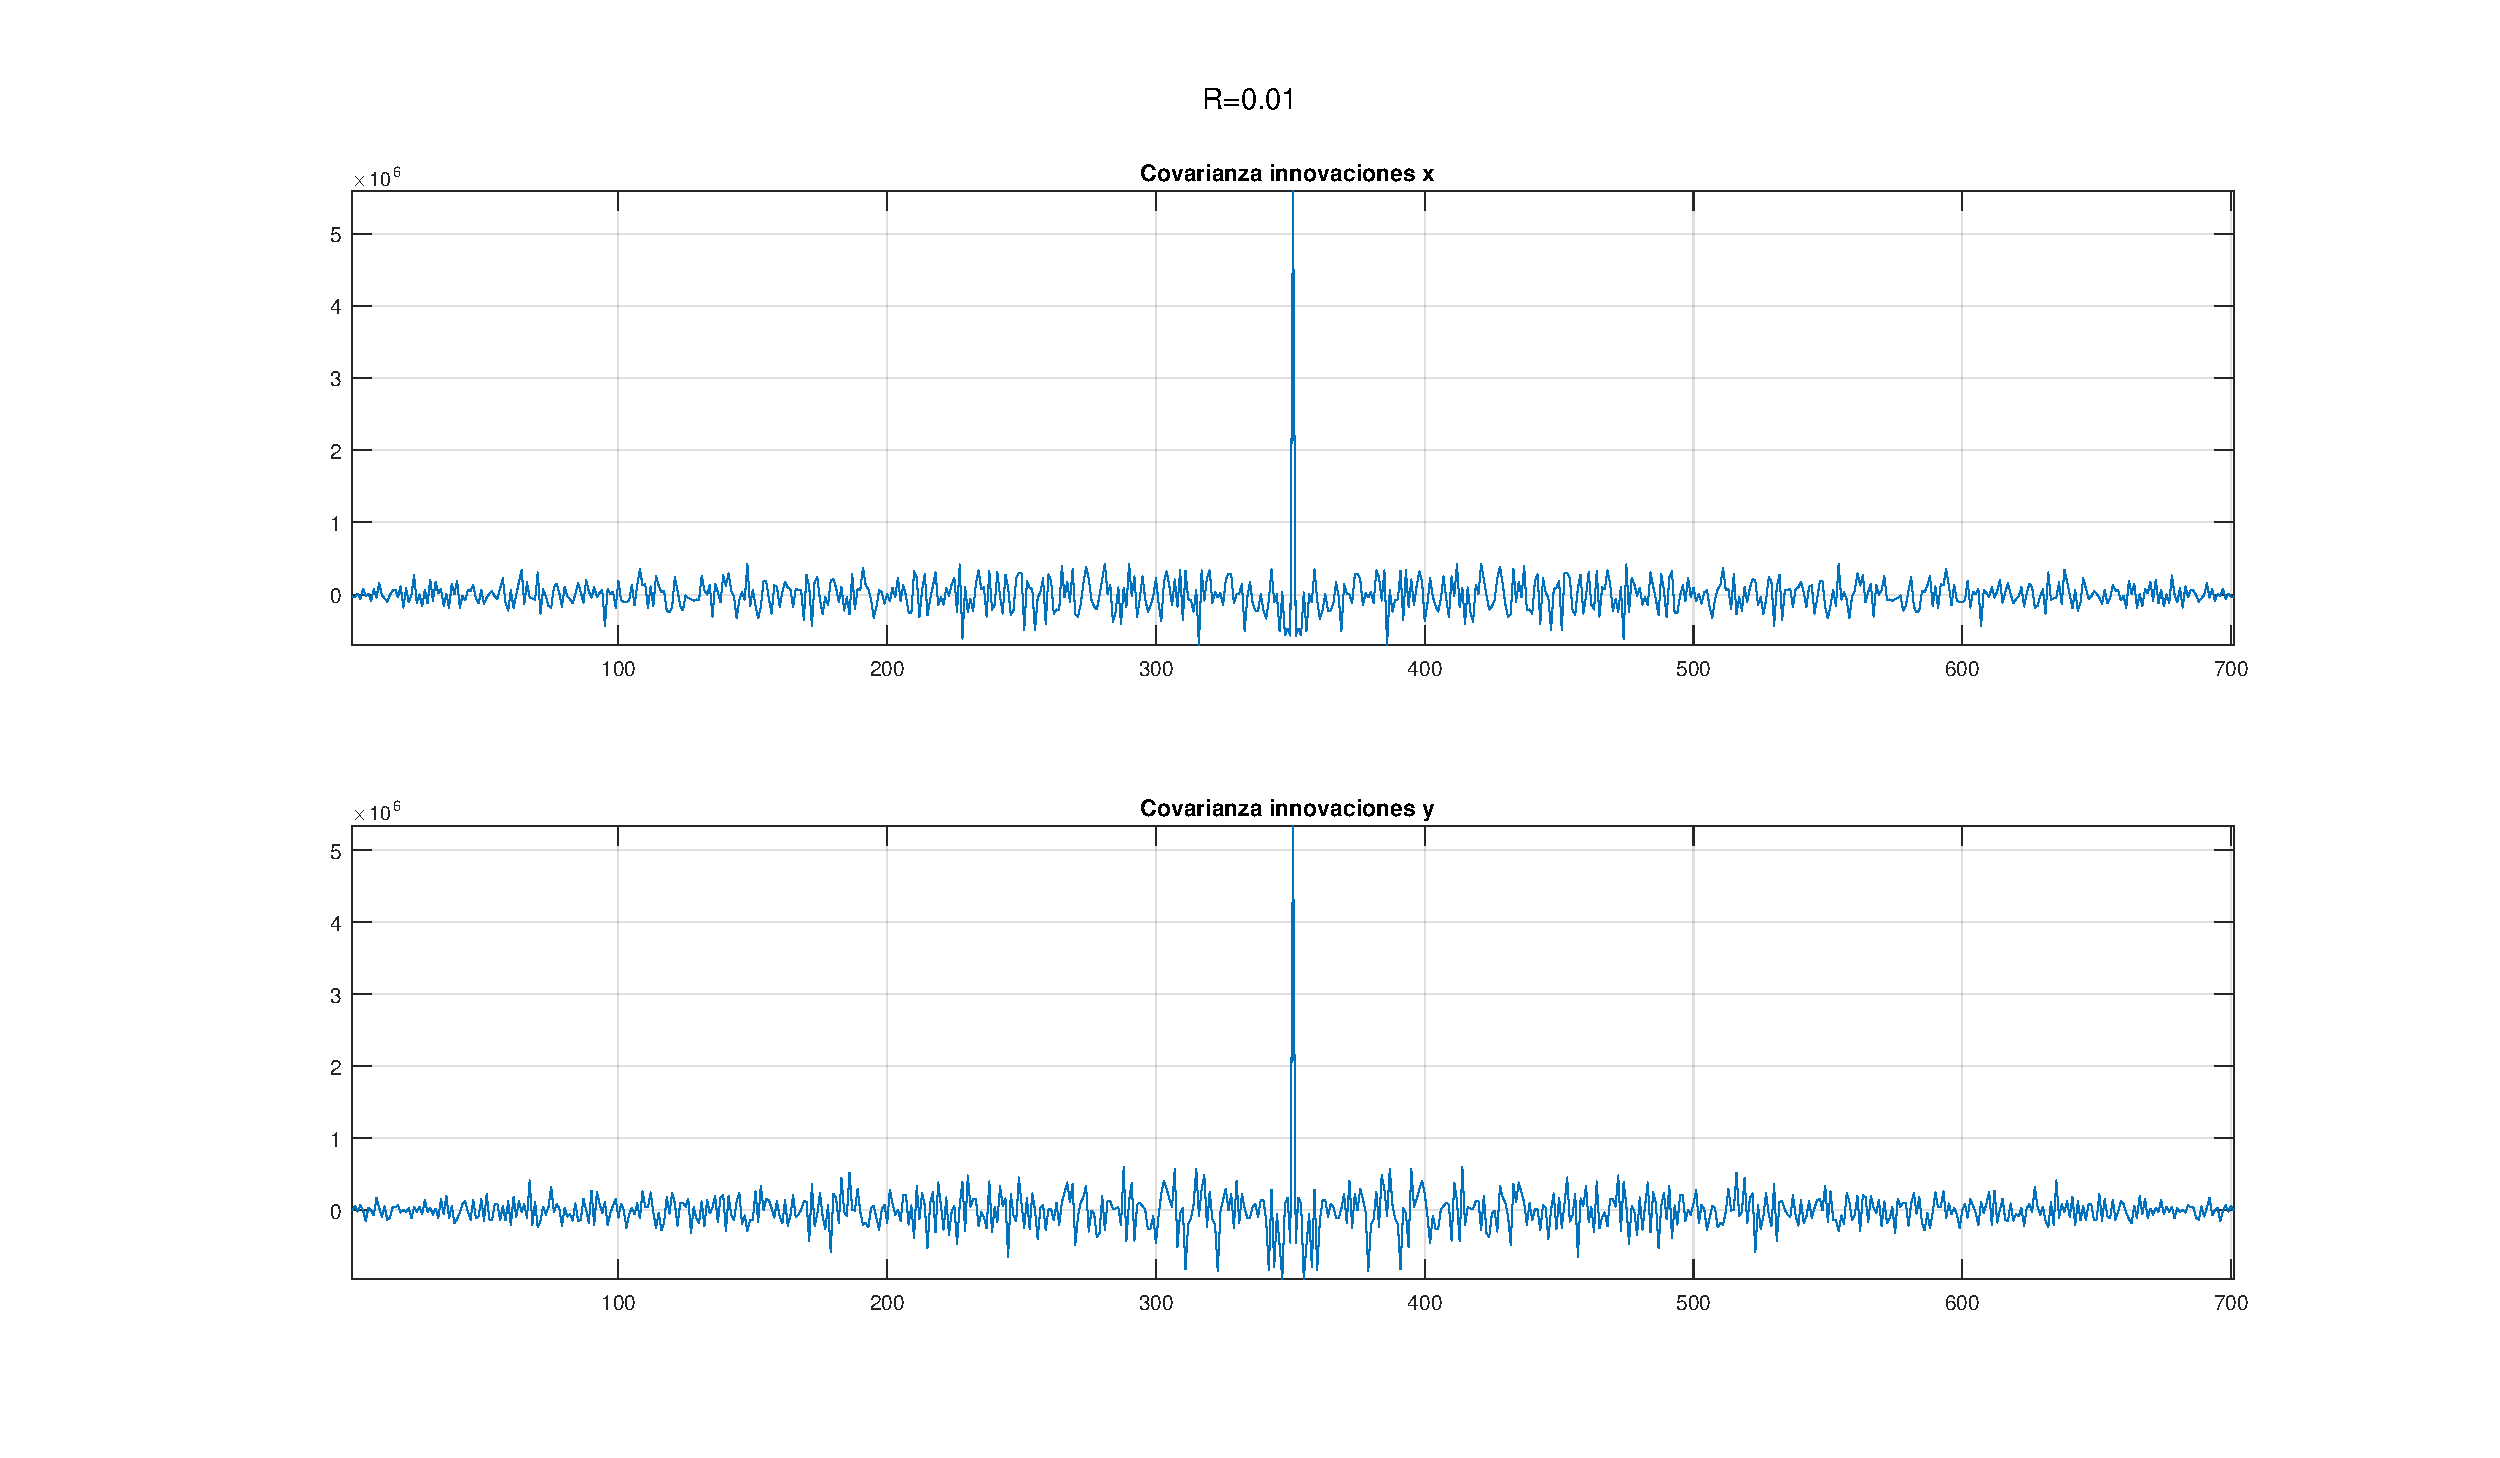
\includegraphics[width=1.0\textwidth,keepaspectratio]{Figuras/covinn_ej6_R2.pdf}
		\caption{Autocorrelación de Innovaciones - Matriz de Covarianza Mayor}
		\label{fig:ej5r2_innov}
	\end{figure}
